% Dit werk is gelicenseerd onder de licentie Creative Commons Naamsvermelding-GelijkDelen 4.0 Internationaal. Ga naar http://creativecommons.org/licenses/by-sa/4.0/ om een kopie van de licentie te kunnen lezen.
\documentclass[t]{beamer}

\usepackage{xcolor}						% Om kleuren te gebruiken
\usepackage[dutch]{babel}               % Voor nederlandstalige hyphenatie (woordsplitsing)
\usepackage{amsmath,amsthm}             % Uitgebreide wiskundige mogelijkheden
\usepackage{url}                        % Om url's te verwerken
\usepackage{graphicx,subfigure}         % Om figuren te kunnen verwerken
\usepackage[utf8]{inputenc}             % Om niet ascii karakters rechtstreeks te kunnen typen
\usepackage{multicol}
\usepackage{listings}					% Code weergeven
\usepackage{courier}					% Code lettertype
\usepackage{textcomp}
\usepackage[absolute,overlay]{textpos}

\lstset{language=Matlab,
        basicstyle=\footnotesize\ttfamily,
        tabsize=4,
        breaklines=true,
        showstringspaces=false,
        upquote=true,
        xleftmargin=0cm,
        xrightmargin=0cm,
        backgroundcolor=\color{black!5!white}}
        
%%%%%%%%%%%%%%%%%%%%%%%%%%%%%%
% Layout
%%%%%%%%%%%%%%%%%%%%%%%%%%%%%%
\usetheme{Frankfurt}
\usefonttheme[onlymath]{serif}
\AtBeginSection[]
{
  \begin{frame}
    \frametitle{Inhoud}
    \tableofcontents[currentsection]
  \end{frame}
}

\setbeamertemplate{navigation symbols}{}

%%%%%%%%%%%%%%%%%%%%%%%%%%%%%%
% Title
%%%%%%%%%%%%%%%%%%%%%%%%%%%%%%
\title{Inleiding tot Matlab}
\author{Brecht Baeten\inst{1}}
\institute{
	\inst{1}%
  		KU Leuven, Technologie campus Diepenbeek,\\ e-mail: brecht.baeten@kuleuven.be
}
\date{\today}

\subtitle{}


\begin{document}
\frame{\titlepage}
\begin{frame}
	\frametitle{Wat is Matlab?}
	\begin{textblock}{6}(8,3)
            
\includegraphics[width=6cm]{fig/matlablogo}
        \end{textblock}
	
	\vspace{1cm}
	
	\begin{itemize}
		\item MATrix LABoratory
		\item Matlab scripting taal
		\item GUI
		\item Toolboxen
	\end{itemize}
\end{frame}
%%%%%%%%%%%%%%%%%%%%%%%%%%%%%%%%%%%%%%%%%%%%%%%%%%%%%%%%%%%%%%%%%%%%%%%%%%%%%%%%%
\begin{frame}
	\frametitle{GUI}
	
	\vspace{-0.9cm}
	
    \center
    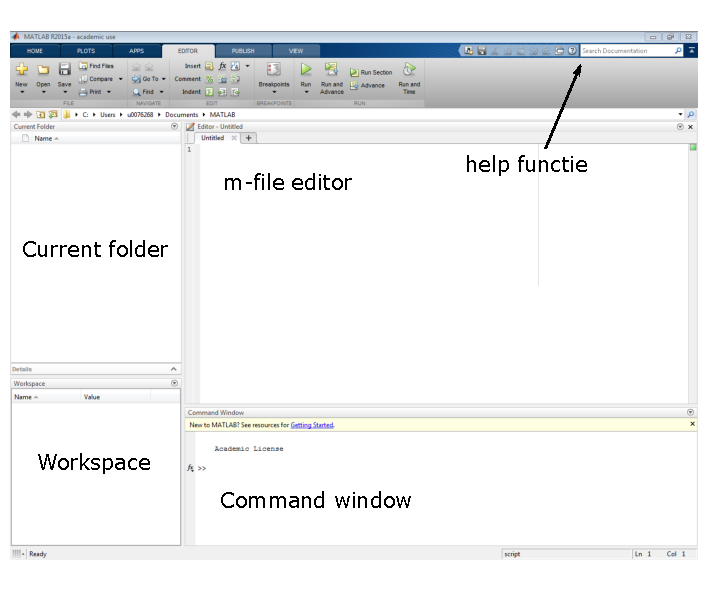
\includegraphics[height=\textheight]{fig/workspace}
    
\end{frame}
%%%%%%%%%%%%%%%%%%%%%%%%%%%%%%%%%%%%%%%%%%%%%%%%%%%%%%%%%%%%%%%%%%%%%%%%%%%%%%%%%
\begin{frame}[fragile]
	\frametitle{Command window}
    \begin{textblock}{6}(8,3)
        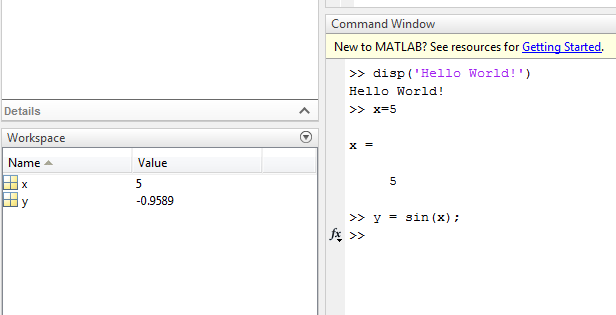
\includegraphics[width=6cm]{fig/commandwindow}
    \end{textblock}
    	
    \begin{itemize}
		\item Commando's uitvoeren
		\item variabelen definieren
		\item functies aanroepen
		\item "\lstinline{;}" verbergt output
		\item Beschikbare variablelen\\ in Workspace
	\end{itemize}
	
    \vspace{0.5cm}
    
	\begin{lstlisting}
>> disp('Hello World!')
>> x = 5
>> x
>> y = sin(x);
>> clear;
>> close all;
>> clc;
	\end{lstlisting}
\end{frame}
%%%%%%%%%%%%%%%%%%%%%%%%%%%%%%%%%%%%%%%%%%%%%%%%%%%%%%%%%%%%%%%%%%%%%%%%%%%%%%%%%
\begin{frame}[fragile]
	\frametitle{Scripts}
	\begin{textblock}{6}(8,3)
        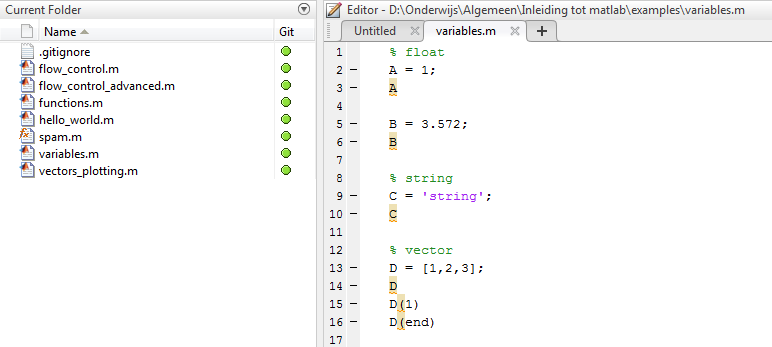
\includegraphics[width=6cm]{fig/available}
    \end{textblock}
    
	\begin{itemize}
		\item Opeenvolgende commando's\\ opgeslagen in een m-file
		\item Aanroepen vanuit het \\command window of vanuit \\m-file editor
		\item Deschikbaar zijn in de \\Current folder of in het \\Matlab pad
	\end{itemize}
	
	\vspace{1cm}
	
	\begin{lstlisting}
>> addpath('lib')
	\end{lstlisting}
\end{frame}
%%%%%%%%%%%%%%%%%%%%%%%%%%%%%%%%%%%%%%%%%%%%%%%%%%%%%%%%%%%%%%%%%%%%%%%%%%%%%%%%%
\begin{frame}[fragile]
	\frametitle{Variabelen}

	\begin{itemize}
		\item Float
		\item Array
		\item String
		\item Cell array
		\item Struct
	\end{itemize}
	
	\begin{lstlisting}
>> B = 3.572;
>> C = 'string';
>> D = [1,2,3];
>> D(1)
>> D(end)

>> E = {1,'test',4,D};

>> F = struct('value',1, 'name','test', 'spam','eggs');
>> F.spam
	\end{lstlisting}
	
\end{frame}
%%%%%%%%%%%%%%%%%%%%%%%%%%%%%%%%%%%%%%%%%%%%%%%%%%%%%%%%%%%%%%%%%%%%%%%%%%%%%%%%%
\begin{frame}
	\frametitle{Controle structuren}
	
	\begin{itemize}
		\item for  end
		\item if  else  end
		\item ...
	\end{itemize}
	
	\vspace{1cm}
		
	\lstinputlisting{examples/flow_control.m}
\end{frame}
%%%%%%%%%%%%%%%%%%%%%%%%%%%%%%%%%%%%%%%%%%%%%%%%%%%%%%%%%%%%%%%%%%%%%%%%%%%%%%%%%
\begin{frame}[fragile]
	\frametitle{Werken met arrays}
	
	\begin{itemize}
		\item prealloceren met "\lstinline{zeros}", "\lstinline{linspace}",...
		\item "\lstinline{length}", "\lstinline{size}"
		\item indexeren met "\lstinline{()}", "\lstinline{:}", "\lstinline{end}"
	\end{itemize}
	
	\begin{lstlisting}
x = zeros(10,1);
for i=1:length(x)
    x(i) = 5*i-2;
end

z = linspace(4,8,20);

y = zeros(10,4);
for i=1:size(y,1)
	for j=1:size(y,2)
    	y(i,j) = 4*i+3*j-2;
    end
end
y(5,2:end)
	\end{lstlisting}
\end{frame}
%%%%%%%%%%%%%%%%%%%%%%%%%%%%%%%%%%%%%%%%%%%%%%%%%%%%%%%%%%%%%%%%%%%%%%%%%%%%%%%%%
\begin{frame}[fragile]
	\frametitle{Functies}
\begin{onlyenv}<1>
	\begin{itemize}
		\item Groeperen van vaak gebruikte commando's
		\item Appart m-file met dezelfde naam als de functie
		\item Documentatie
	\end{itemize}

	\begin{lstlisting}
function val = digits2number(A,B,C,D)
	% returns a a number as if the arguments were different digits in the
	number
	%
	% Parameters:
	% A: float, hundreds
	% B: float, decades
	% C: float, units
	% D: float, tenths
	
	val = 100*A+10*B+C+0.1*D;
end
	\end{lstlisting}
\end{onlyenv}
\begin{onlyenv}<2>
	\center
	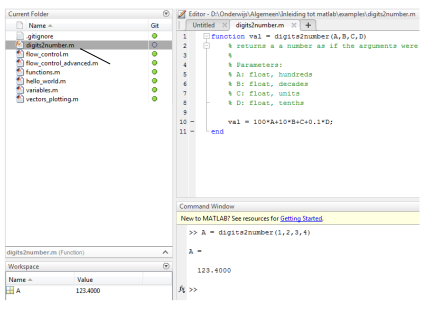
\includegraphics[height=0.8\textheight]{fig/functie}
\end{onlyenv}
\end{frame}
%%%%%%%%%%%%%%%%%%%%%%%%%%%%%%%%%%%%%%%%%%%%%%%%%%%%%%%%%%%%%%%%%%%%%%%%%%%%%%%%%
\begin{frame}[fragile]
	\frametitle{Plotten}
	\begin{itemize}
		\item "\lstinline{figure}", "\lstinline{plot}", "\lstinline{hold}", "\lstinline{xlabel}", "\lstinline{legend}", "\lstinline{grid}"
		\item Gebruik \LaTeX\ om labels en legendes weer te geven
	\end{itemize}

	\begin{lstlisting}
x = linspace(0,2 * pi,50);
s = sin(x);
c = cumtrapz(x,s);

figure('Position', [100, 100, 400, 280]);
hold on; grid on;
plot(x,c,'r','linewidth',2);
xlabel('$x$ (rad)','Interpreter','latex');
ylabel('$y$','Interpreter','latex');
legend({'$\int$ sinus(x) d$x$'},'Interpreter','latex');

set(gcf,'units','centimeters')
set(gcf,'papersize',[8,5])
set(gcf,'paperposition',[0,0,8,5])
print('sinus_cosinus','-dpdf')
print('sinus_cosinus','png')
	\end{lstlisting}
\end{frame}
%%%%%%%%%%%%%%%%%%%%%%%%%%%%%%%%%%%%%%%%%%%%%%%%%%%%%%%%%%%%%%%%%%%%%%%%%%%%%%%%%
\begin{frame}
	\frametitle{Bestanden inlezen}
\begin{onlyenv}<1>
	\begin{itemize}
		\item Gebruik de wizard
		\item Gebruik de wizard
		\item Gebruik de wizard!
	\end{itemize}
	
	\center
	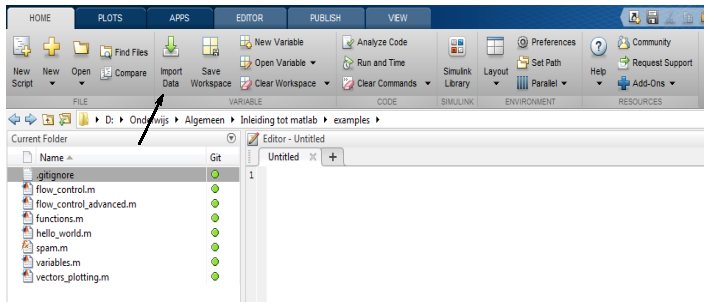
\includegraphics[height=0.5\textheight]{fig/import}
	
\end{onlyenv}
\begin{onlyenv}<2>

	\center
	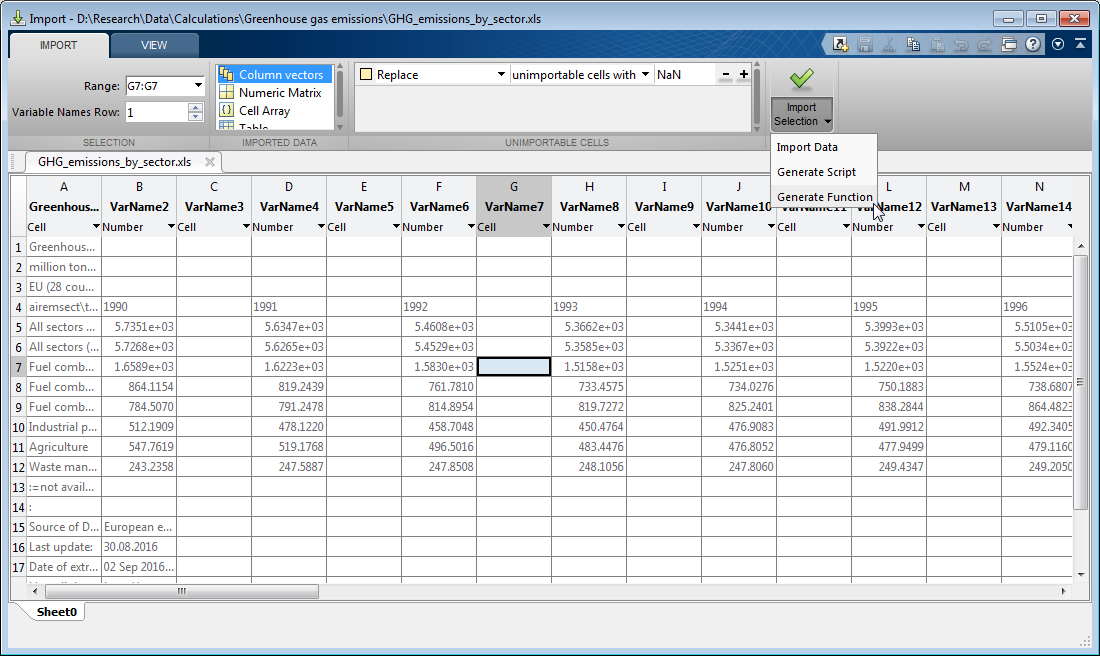
\includegraphics[width=\textwidth]{fig/importwizard}
	
\end{onlyenv}
\end{frame}  	
%%%%%%%%%%%%%%%%%%%%%%%%%%%%%%%%%%%%%%%%%%%%%%%%%%%%%%%%%%%%%%%%%%%%%%%%%%%%%%%%%
\begin{frame}[fragile]
	\frametitle{Een project structureren}
\begin{onlyenv}<1>
	\begin{itemize}
		\item Gebruik functies
		\item Maak binnen functies gebruik van sub-functies indien nuttig
		\item Geef functies een betekenisvolle naam
		\item Groepeer functies die bij elkaar horen in een map en voeg deze map toe aan het Matlab pad
		\item Don't Repeat Yourself (DRY)
		\item Gebruik betekenisvolle namen voor variabelen
		\item Documenteer alles
	\end{itemize}
\end{onlyenv}
\begin{onlyenv}<2>
Voorbeeld folderstructuur:

	\begin{lstlisting}[language=bash]
mijnProject	
|-- data
|   |-- mijndata.csv
|
|-- lib
|   |-- data
|   |   |-- data_inlezen.m
|   |   |-- data_naar_coordinaten.m
|   |
|   |-- plot
|       |-- plot_coordinaten.m
|
|-- main.m
|
|-- readme
	\end{lstlisting}
\end{onlyenv}
\begin{onlyenv}<3>

Voorbeeld main.m:
	\begin{lstlisting}
% main.m
% dit script leest data in, vertaalt deze in coordinaten
% en maakt een plot

% de workspace leegmaken
clear; clc; close all;

% functies toevoegen aan het pad
addpath('lib/data');
addpath('lib/plot');

% data inlezen en bewerken
data = data_inlezen('data/mijndata.csv');
[x,y,z] = data_naar_coordinaten(data);

% plotten
plot_coordinaten(x,y,z);
	\end{lstlisting}	
	
\end{onlyenv}
\end{frame}
%%%%%%%%%%%%%%%%%%%%%%%%%%%%%%%%%%%%%%%%%%%%%%%%%%%%%%%%%%%%%%%%%%%%%%%%%%%%%%%%%
\begin{frame}
	\footnotesize
	\vspace{4cm}
	\includegraphics[height=0.3cm]{fig/cc} \
	\includegraphics[height=0.3cm]{fig/by} \
	\includegraphics[height=0.3cm]{fig/sa}
	\quad \the\year\ Brecht Baeten
	\vspace{0.5cm}
	
    Dit werk is gelicenseerd onder de licentie Creative Commons Naamsvermelding-GelijkDelen 4.0 Internationaal. Ga naar http://creativecommons.org/licenses/by-sa/4.0/ om een kopie van de licentie te kunnen lezen.
    	
    \vspace{0.5cm}
    De bron van dit document en alle tekeningen zijn beschikbaar op https://github.com/BrechtBa/inleiding-tot-matlab
\end{frame}
%%%%%%%%%%%%%%%%%%%%%%%%%%%%%%%%%%%%%%%%%%%%%%%%%%%%%%%%%%%%%%%%%%%%%%%%%%%%%%%%%	
\end{document}